\section{Electronics}
\label{electronics}
The finger drums prototype will consist of 5 force sensitive resistors connected to the analog pins of an Arduino Uno. The FSRs used in this prototype will be an FSR-152. In order to get the desired output signal from the FSR it is connected with a normal resistor to create a voltage divider as seen in \autoref{fig:simple_voltage_divider}. 
\begin{figure}[H]
\centering
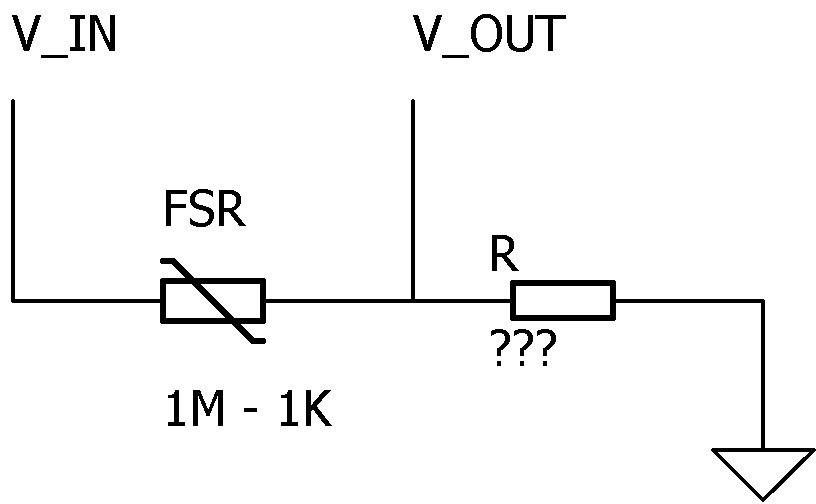
\includegraphics[scale=1.5]{Figure/simple_voltage_divider.png}
\caption{Simple voltage divider with the FSR represented as a variable resistor. }
\label{fig:simple_voltage_divider}
\end{figure}

In order to find a fitting value for the resistor R the formula for a voltage divider is used, \autoref{fig:R_calculation}.
\begin{figure}[H]
\centering
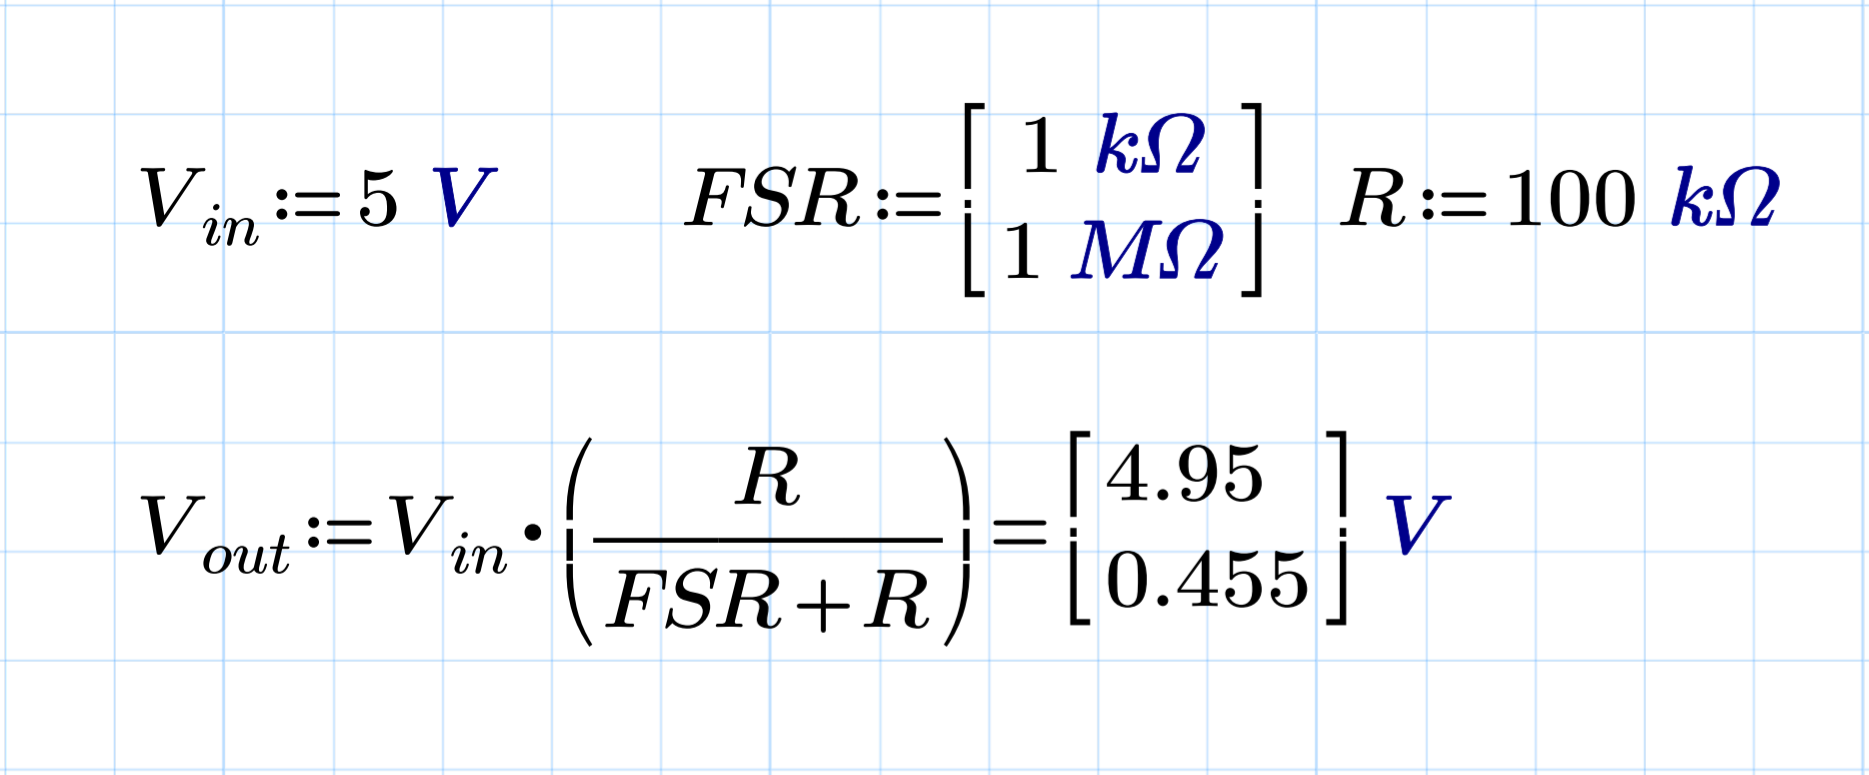
\includegraphics[scale=0.15]{Figure/R_calculation.png}
\caption{Calculation of a voltage divider.}
\label{fig:R_calculation}
\end{figure}

The input voltage from the Arduino is 5V, the FSR varies in the range 1 M$\Omega$ to 1 K$\Omega$, and the ideal output voltage is around 0V and 5V depending on the value of the FSR. From \autoref{fig:R_calculation} a resistor of 100 K$\Omega$ is found to be fitting resulting in an output voltage that will range form 4.95V to 0.455V, assuming all components are ideal. The final circuit diagram, all components included can be seen in \autoref{fig:Schematic2}. 
\begin{figure}[H]
\centering
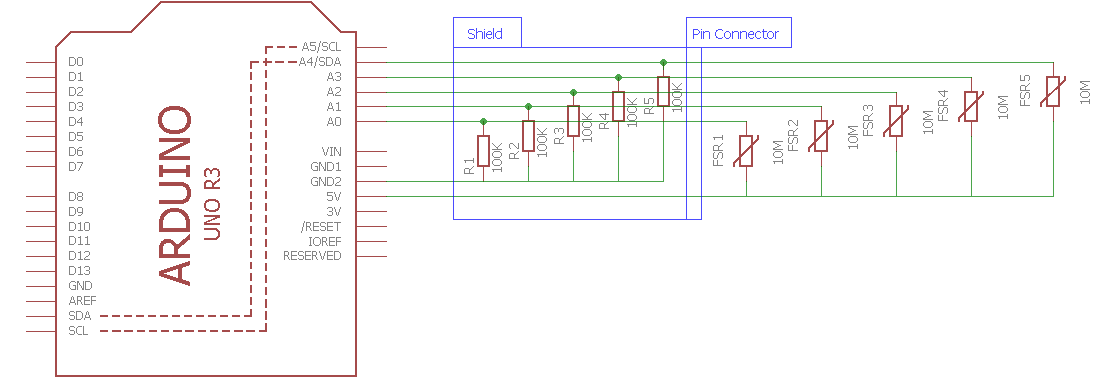
\includegraphics[scale=0.5]{Figure/Schematic2.png}
\caption{Schematic for the final circuit with the blue box indicating which components are actually on the shield.}
\label{fig:Schematic2}
\end{figure}

The next step was to build an actual shield that would fit over the Arduino and connect to the sensors can then be put in a glove. As this is just a prototype the shield was just made from a piece of through hole prototyping board cut down to a reasonable size and with pins soldered in on both sides to help get a solid connection with the Arduino.

**Billede af shield**

The shield could also be made as a printed circuit board in which case it could look like \autoref{fig:TopBottomPCB}, here routed on both top and bottom side of the PCB in order to avoid collisions of paths and a to maintain clarity.
\begin{figure}[H]
\centering
\includegraphics[scale=0.15]{Figure/TopBottomPCB.png}
\caption{An example of how the shield could be routed on PCB. Left is the top of the board, right is the bottom.}
\label{fig:TopBottomPCB}
\end{figure}